\section{Revision Exercise 26}

\begin{enumerate}
    \item Find the equation of the tangent of the curve $y = x^3 - 3x$ at the point where
          $x = 3$. \sol{}
          \begin{flalign*}
              y              & = x^3 - 3x & \\
              \dfrac{dy}{dx} & = 3x^2 - 3
          \end{flalign*}
          At $x = 3$, $y = (3)^3 - 3(3) = 18$.
          \begin{flalign*}
              \text{Gradient of tangent }\dfrac{dy}{dx}        & = 3(3)^2 - 3 & \\
                                                               & = 27 - 3     & \\
                                                               & = 24         & \\
              \therefore\ \text{Equation of tangent is }y - 18 & = 24(x - 3)  & \\
              y - 18                                           & = 24x - 72   & \\
              y                                                & = 24x - 54
          \end{flalign*}
          \vfill\null

    \item Find the equation of the normal of the curve $y = x(x-4)(x+1)$ at the points of
          intersection of the curve and the $x$-axis. \sol{} \vspace{-2em}
          \begin{multicols}{2}
              \begin{flalign*}
                  y              & = x(x-4)(x+1)     & \\
                                 & = x(x^2 - 3x - 4) & \\
                                 & = x^3 - 3x^2 - 4x & \\
                  \dfrac{dy}{dx} & = 3x^2 - 6x - 4
              \end{flalign*}
              \vspace{-2em}
              \begin{flalign*}
                  \text{When } x = 0, y & = 0                    & \\
                  x(x-4)(x+1)           & = 0                    & \\
                  x = 0 \text{ or } x   & = 4 \text{ or } x = -1
              \end{flalign*}
              When $x = 0$,
              \begin{flalign*}
                  \because\ \text{Gradient of tangent }\dfrac{dy}{dx} & = 3(0)^2 - 6(0) - 4 = -4 & \\
                  \therefore\ \text{Gradient of normal }              & = \dfrac{1}{4}           & \\
                  \therefore\ \text{Equation of normal is }y - 0      & = \dfrac{1}{4}(x - 0)    & \\
                  y                                                   & = \dfrac{1}{4}x          & \\
                  x - 4y                                              & = 0
              \end{flalign*}
              \vfill{}\null{}
              When $x = 4$,
              \begin{flalign*}
                  \because\ \text{Gradient of tangent }\dfrac{dy}{dx} & = 3(4)^2 - 6(4) - 4 = 20 & \\
                  \therefore\ \text{Gradient of normal }              & = -\dfrac{1}{20}         & \\
                  \therefore\ \text{Equation of normal is }y - 0      & = -\dfrac{1}{20}(x - 4)  & \\
                  x + 20y -4                                          & = 0
              \end{flalign*}
              When $x = -1$,
              \begin{flalign*}
                  \because\ \text{Gradient of tangent }\dfrac{dy}{dx} & = 3(-1)^2 - 6(-1) - 4 = 5 & \\
                  \therefore\ \text{Gradient of normal }              & = -\dfrac{1}{5}           & \\
                  \therefore\ \text{Equation of normal is }y - 0      & = -\dfrac{1}{5}(x + 1)    & \\
                  x + 5y + 1                                          & = 0
              \end{flalign*}
              \vfill{}\null{}
          \end{multicols}
          Hence, the equations of the normals are $x - 4y = 0$, $x + 20y - 4 = 0$ and $x + 5y + 1 = 0$.
          \vfill\null

          \newpage
          \setlength{\columnsep}{1cm}
          \begin{multicols}{2}
              \item Given that the curve $y = ax^2 + bx - 10$ passes through the point $(2, 0)$,
              and that the gradient of the curve at the point is $3$. Find the values of $a$
              and $b$. \sol{}
              \begin{flalign*}
                  y              & = ax^2 + bx - 10 & \\
                  \dfrac{dy}{dx} & = 2ax + b
              \end{flalign*}
              Since the curve passes through $(2, 0)$,
              \begin{flalign*}
                  0  & = a(2)^2 + b(2) - 10                 & \\
                  0  & = 4a + 2b - 10                       & \\
                  4a & = 10 - 2b                            & \\
                  a  & = \dfrac{10 - 2b}{4}                 & \\
                     & = \dfrac{5 - b}{2} \quad \cdots\ (1)
              \end{flalign*}
              Since the gradient of the curve at the point is $3$,
              \begin{flalign*}
                  3 & = 2a(2) + b                & \\
                  3 & = 4a + b \quad \cdots\ (2)
              \end{flalign*}
              Substituting $(1)$ into $(2)$,
              \begin{flalign*}
                  3 & = 4\left(\dfrac{5 - b}{2}\right) + b & \\
                  3 & = 2(5 - b) + b                       & \\
                  3 & = 10 - 2b + b                        & \\
                  b & = 7
              \end{flalign*}
              Substituting $b = 7$ into $(1)$,
              \begin{flalign*}
                  a & = \dfrac{5 - 7}{2} & \\
                    & = -1
              \end{flalign*}
              Hence, $a = -1$ and $b = 7$.
              \vfill{}\null{}
              \item Find the equation of the normal of the curve $y = x + \dfrac{2}{x}$ at the
              point $(2, 3)$. If the normal line intersects with the $x$-axis and $y$-axis at
              $A$ and $B$ respectively, find the length of $AB$. \sol{}
              \begin{flalign*}
                  y              & = x + \dfrac{2}{x}   & \\
                  \dfrac{dy}{dx} & = 1 - \dfrac{2}{x^2}
              \end{flalign*}
              At $x = 2$,
              \begin{flalign*}
                  \dfrac{dy}{dx} & = 1 - \dfrac{2}{2^2} & \\
                                 & = \dfrac{1}{2}
              \end{flalign*}
              Hence, the gradient of the normal at the point $(2, 3)$ is $-2$.

              Therefore, the equation of the normal is
              \begin{flalign*}
                  y - 3 & = -2(x - 2) & \\
                  y     & = -2x + 7
              \end{flalign*}
              When $y = 0$,
              \begin{flalign*}
                  0             & = -2x + 7                      & \\
                  x             & = \dfrac{7}{2}                 & \\
                  \therefore\ A & = \left(\dfrac{7}{2}, 0\right)
              \end{flalign*}
              When $x = 0$,
              \begin{flalign*}
                  y             & = -2(0) + 7         & \\
                  y             & = 7                 & \\
                  \therefore\ B & = \left(0, 7\right)
              \end{flalign*}
              \begin{flalign*}
                  AB & = \sqrt{\left(\dfrac{7}{2} - 0\right)^2 + \left(0 - 7\right)^2} & \\
                     & = \sqrt{\dfrac{49}{4} + 49}                                     & \\
                     & = \sqrt{\dfrac{245}{4}}                                         & \\
                     & = \dfrac{\sqrt{245}}{2}                                         & \\
                     & = \dfrac{7\sqrt{5}}{2}
              \end{flalign*}
              \vfill{}\null{}
          \end{multicols}
\end{enumerate}
\newpage
\noindent \hspace{1.2em}\textit{Of the following functions, which intervals are the function increasing or decreasing? (Question 5 to 6)}
\begin{enumerate}
    \setcounter{enumi}{4}
    \item $f(x) = 2x^2(6-x)$
          \sol{}
          \begin{flalign*}
              f(x)       & = 2x^2(6-x)       & \\
                         & = 12x^2 - 2x^3    & \\
              f'(x)      & = 24x - 6x^2      & \\
              f'(x)      & = 0               & \\
              24x - 6x^2 & = 0               & \\
              x(x - 4)   & = 0               & \\
              x = 0      & \text{ or } x = 4
          \end{flalign*}
          At the interval $(-\infty, 0)$, $f'(x) < 0$, hence $f(x)$ is decreasing at the interval $(-\infty, 0]$.

          At the interval $(0, 4)$, $f'(x) > 0$, hence $f(x)$ is increasing at the
          interval $[0, 4]$.

          At the interval $(4, \infty)$, $f'(x) < 0$, hence $f(x)$ is decreasing at the
          interval $[4, \infty)$. \vfill\null

    \item $f(x) = 4x^3 - 3x^2 - 6x + 1$
          \sol{}
          \begin{flalign*}
              f(x)              & = 4x^3 - 3x^2 - 6x + 1 & \\
              f'(x)             & = 12x^2 - 6x - 6       & \\
              f'(x)             & = 0                    & \\
              12x^2 - 6x - 6    & = 0                    & \\
              2x^2 - x - 1      & = 0                    & \\
              (2x + 1)(x - 1)   & = 0                    & \\
              x = -\dfrac{1}{2} & \text{ or } x = 1
          \end{flalign*}
          At the interval $\left(-\infty, -\dfrac{1}{2}\right)$, $f'(x) > 0$, hence $f(x)$ is increasing at the interval $\left.\left(-\infty, -\dfrac{1}{2}\right]\right.$.

          At the interval $\left(-\dfrac{1}{2}, 1\right)$, $f'(x) < 0$, hence $f(x)$ is
          decreasing at the interval $\left.\left[-\dfrac{1}{2}, 1\right]\right.$.

          At the interval $\left(1, \infty\right)$, $f'(x) > 0$, hence $f(x)$ is
          increasing at the interval $\left.\left[1, \infty\right)\right.$. \vfill\null

          \newpage
          \begin{multicols}{2}
              \item If $x - y = 3$, find the relative minimum value of $x^2y$. \sol{}
              \begin{flalign*}
                  x - y & = 3     & \\
                  y     & = x - 3
              \end{flalign*}
              Let $f(x) = x^2y$,
              \begin{flalign*}
                  f(x)      & = x^2y            & \\
                            & = x^2(x - 3)      & \\
                            & = x^3 - 3x^2      & \\
                  f'(x)     & = 3x^2 - 6x       & \\
                  f'(x)     & = 0               & \\
                  3x^2 - 6x & = 0               & \\
                  x(x - 2)  & = 0               & \\
                  x = 0     & \text{ or } x = 2
              \end{flalign*}
              \vspace{-3em}
              \begin{flalign*}
                   & f''(x)            = 6x - 6                                 & \\
                   & \because\ f''(0)  = -6 < 0,\ f''(2) = 6 > 0                & \\
                   & \therefore\ f(2) = -4 \text{ is a relative minimum value.}
              \end{flalign*}

              \item If $2x^2 + y^2 = 6x$, find the relative maximum value of $x^2 + y^2 + 2x$.
              \sol{}
              \begin{flalign*}
                  2x^2 + y^2 & = 6x        & \\
                  y^2        & = 6x - 2x^2
              \end{flalign*}
              Let $f(x) = x^2 + y^2 + 2x$,
              \begin{flalign*}
                  f(x)    & = x^2 + y^2 + 2x       & \\
                          & = x^2 + 6x - 2x^2 + 2x & \\
                          & = -x^2 + 8x            & \\
                  f'(x)   & = -2x + 8              & \\
                  f'(x)   & = 0                    & \\
                  -2x + 8 & = 0                    & \\
                  x - 4   & = 0                    & \\
                  x = 4
              \end{flalign*}
              \vspace{-3em}
              \begin{flalign*}
                   & f''(x)            = -2                                     & \\
                   & \because\ f''(4)  = -2 < 0                                 & \\
                   & \therefore\ f(4) = 16 \text{ is a relative maximum value.}
              \end{flalign*}
          \end{multicols}
          \vfill\null

    \item Given that $y = 18x^2 + 12x + 7$ has a relative minimum value $q$ and the point
          where $x = p$. Find the value of $p$ and $q$. \sol{}
          \begin{flalign*}
              y        & = 18x^2 + 12x + 7 & \\
              y'       & = 36x + 12        & \\
              y'       & = 0               & \\
              36x + 12 & = 0               & \\
              3x + 1   & = 0               & \\
              p =  x   & = -\dfrac{1}{3}
          \end{flalign*}
          \vspace{-3em}
          \begin{flalign*}
               & \text{When }x = -\dfrac{1}{3},\ y = 5                   & \\
               & y''            = 36 > 0                                 & \\
               & \therefore\ \text{The relative minimum value is }q = 5.
          \end{flalign*}
          \vfill\null

          \newpage
    \item There's a rectangular field where one side of it is a wall and the other three
          sides are fenced. If the total length of the fence is $40m$, find the width and
          height of the field such that the area of the field is the maximum. \sol{} Let
          $x$ be the length of the field and $y$ be the width of the field.
          \begin{flalign*}
              2x + y         & = 40         & \\
              y              & = 40 - 2x    & \\
              A              & = xy         & \\
                             & = x(40 - 2x) & \\
                             & = 40x - 2x^2 & \\
              \dfrac{dA}{dx} & = 40 - 4x    & \\
              \dfrac{dA}{dx} & = 0          & \\
              40 - 4x        & = 0          & \\
              x              & = 10
          \end{flalign*}
          \vspace{-3em}
          \begin{flalign*}
               & \because\ \dfrac{d^2A}{dx^2} = -4 < 0                                                                            & \\
               & \therefore\ \text{The area of the field is the maximum when }x = 10. \text{When } x = 10,\ y = 20.               & \\
               & \therefore\ \text{The field has a width of }20m\text{ and a height of }10m \text{ when the area is the maximum.}
          \end{flalign*}

    \item One side of a rectangle with a perimeter of $18cm$ is revolved about one side
          to form a cylinder. If the volume of the cylinder is the maximum, find the
          dimensions of the rectangle and the maximum volume of the cylinder. \sol{}

          Let the length of the rectangle be $x$ and the width of the rectangle be $y$.
          \begin{flalign*}
              2x + 2y & = 18    & \\
              x + y   & = 9     & \\
              y       & = 9 - x
          \end{flalign*}
          \vspace{-3em}
          \begin{flalign*}
              V               & = \pi r^2 h                                   & \\
                              & = \pi x^2y                                    & \\
                              & = \pi(9x^2 - x^3)                             & \\
              \dfrac{dV}{dx}  & = \pi(18x - 3x^2)                             & \\
              \dfrac{dV}{dx}  & = 0                                           & \\
              \pi(18x - 3x^2) & = 0                                           & \\
              x^2 - 6x        & = 0                                           & \\
              x(x - 6)        & = 0                                           & \\
              x = 6           & ,\ x        = 0   \text{ (rejected, $x > 0$)}
          \end{flalign*}
          \vspace{-3em}
          \begin{flalign*}
               & \because\ \dfrac{d^2V}{dx^2} = \pi(18 - 6x) = -18\pi < 0                                                                         & \\
               & \therefore\ \text{The volume of the cylinder is the maximum when }x = 6. \text{When } x = 6,\ y = 3.                             & \\
               & \therefore\ \text{The rectangle has a length of }6cm\text{ and a width of }3cm \text{ when the volume is the maximum.}           & \\
               & \text{Also, the maximum volume of the cylinder is }V = \pi(6)^2(3) = 108\pi \text{ cm}^3 \text{ when the volume is the maximum.}
          \end{flalign*}

          \newpage
    \item The cross section of a tunnel is a rectangle with a semicircle on top of it. If
          the area of the cross section is fixed, find the ratio of the radius of the
          semicircle to the height of the rectangle such that the perimeter of the cross
          section is the minimum. \sol{}

          Let the radius of the semicircle be $r$ and the height of the rectangle be $h$.
          \begin{flalign*}
              A                                                                                 & = \dfrac{1}{2}\pi r^2 + 2rh                     & \\
              2rh                                                                               & = A - \dfrac{1}{2}\pi r^2                       & \\
              h                                                                                 & = \dfrac{A - \dfrac{1}{2}\pi r^2}{2r}           & \\
                                                                                                & = \dfrac{A}{2r} - \dfrac{1}{4}\pi r             & \\
              P                                                                                 & = \pi r + 2h + 2r                               & \\
                                                                                                & = (\pi + 2)r + \dfrac{A}{r} - \dfrac{1}{2}\pi r & \\
              \dfrac{dP}{dr}                                                                    & = \pi + 2 - \dfrac{A}{r^2} - \dfrac{1}{2}\pi    & \\
                                                                                                & = \dfrac{1}{2}\pi + 2 - \dfrac{A}{r^2}          & \\
              \dfrac{dP}{dr}                                                                    & = 0                                             & \\
              \dfrac{1}{2}\pi + 2 - \dfrac{A}{r^2}                                              & = 0                                             & \\
              \dfrac{1}{2}\pi + 2 - \left(\dfrac{1}{2}\pi r^2 + 2rh\right) \cdot \dfrac{1}{r^2} & = 0                                             & \\
              \dfrac{1}{2}\pi + 2 - \dfrac{1}{2}\pi - \dfrac{2}{r}h                             & = 0                                             & \\
              2 - \dfrac{2}{r}h                                                                 & = 0                                             & \\
              2                                                                                 & = \dfrac{2}{r}h                                 & \\
              2r                                                                                & = 2h                                            & \\
              r                                                                                 & = h
          \end{flalign*}
          Hence, the ratio of the radius of the semicircle to the height of the rectangle is $1:1$.

          \newpage
    \item Split 28 into two parts such that the sum of the squares of the one part and
          the cube of the other part is the minimum. \sol{}

          Let the two parts be $x$ and $y$.
          \begin{flalign*}
              x + y                   & = 28                           & \\
              y                       & = 28 - x                       & \\
              S                       & = x^2 + y^3                    & \\
                                      & = x^2 + {(28 - x)}^3           & \\
              \dfrac{dS}{dx}          & = 2x - 3{(28 - x)}^2           & \\
              \dfrac{dS}{dx}          & = 0                            & \\
              2x - 3{(28 - x)}^2      & = 0                            & \\
              2x - 3(784 - 56x + x^2) & = 0                            & \\
              2x - 2352 + 168x - 3x^2 & = 0                            & \\
              3x^2 - 170x + 2352      & = 0                            & \\
              (3x - 98)(x - 24)       & = 0                            & \\
              x = 24                  & \text{ or }\ x = \dfrac{98}{3}
          \end{flalign*}
          \vspace{-3em}
          \begin{flalign*}
              \dfrac{d^2S}{dx^2} & = 2 + 6(28 - x) & \\
                                 & = 2 + 168 - 6x  & \\
                                 & = -6x + 170
          \end{flalign*}
          \vspace{-3em}
          \begin{flalign*}
              \text{When } x = 24,\ \dfrac{d^2S}{dx^2}            & = -6(24) + 170                       & \\
                                                                  & = 26 > 0                             & \\
              \text{When } x = \dfrac{98}{3},\ \dfrac{d^2S}{dx^2} & = -6\left(\dfrac{98}{3}\right) + 170 & \\
                                                                  & = -26 < 0
          \end{flalign*}
          \vspace{-3em}
          \begin{flalign*}
               & \because\ \text{When } x = 24,\ \dfrac{d^2S}{dx^2} > 0,                                                              & \\
               & \therefore\ \text{The sum of the squares of the one part and the cube of the other part is the minimum when }x = 24. & \\
               & \because\ \text{When } x = 24,\ y = 4.                                                                               & \\
               & \therefore\ \text{The two parts are 24 and 4.}
          \end{flalign*}
          \newpage
    \item The capacity of a cylindrical can is fixed. If the material used to make the
          can is the minimum, what should be the ratio of the radius of the base to the
          height of the can? \sol{}

          Let the radius of the base be $r$ and the height of the can be $h$.
          \begin{flalign*}
              V                        & = \pi r^2h                 & \\
              h                        & = \dfrac{V}{\pi r^2}       & \\
              A                        & = 2\pi r^2 + 2\pi rh       & \\
                                       & = 2\pi r^2 + \dfrac{2V}{r} & \\
              \dfrac{dA}{dr}           & = 4\pi r - \dfrac{2V}{r^2} & \\
              \dfrac{dA}{dr}           & = 0                        & \\
              4\pi r - \dfrac{2V}{r^2} & = 0                        & \\
              2\pi r^3 - \pi r^2h      & = 0                        & \\
              2r^3 - r^2h              & = 0                        & \\
              2r - h                   & = 0                        & \\
              2r                       & = h                        & \\
              \dfrac{r}{h}             & = \dfrac{1}{2}
          \end{flalign*}
          Hence, the ratio of the radius of the base to the height of the can is $1:2$.
\end{enumerate}
\hspace{0.5em} \textit{Find the coordinate of the point of inflection of the following functions. (Question 15 to 16)}
\begin{enumerate}
    \setcounter{enumi}{14}
    \item $y = x^3 - 2$
          \sol{}
          \begin{flalign*}
              y'    & = 3x^2 & \\
              y''   & = 6x   & \\
              6x    & = 0    & \\
              x = 0 &
          \end{flalign*}
          When $x = 0$, $y = -2$.

          Hence, the coordinate of the point of inflection is $(0, -2)$.

    \item $3x + {(2-x)}^3$
          \sol{}
          \begin{flalign*}
              y'     & = 3 - 3{(2-x)}^2 & \\
              y''    & = 6(2-x)         & \\
              6(2-x) & = 0              & \\
              x = 2  &
          \end{flalign*}
          When $x = 2$, $y = 6$.

          Hence, the coordinate of the point of inflection is $(2, 6)$.

    \item Given the function $y = \dfrac{x}{1-x^2}$. Find the extreme values of the
          function, and determine the coordinates of the convex intervals and the point
          of inflection. \sol{}
          \begin{flalign*}
              y'       & = \dfrac{1 - x^2 + 2x^2}{(1-x^2)^2} & \\
                       & = \dfrac{x^2 + 1}{(1-x^2)^2}        & \\
              y'       & = 0                                 & \\
              x^2 + 1  & = 0                                 & \\
              x^2      & = -1                                & \\
              x \notin & \ \mathbb{R}
          \end{flalign*}
          Since $x \notin \mathbb{R}$, there are no extreme values of the function.
          \begin{flalign*}
              y'' & = \dfrac{2x(1-x^2)^2 + 2(x^2 + 1)(2x)(1-x^2)}{(1-x^2)^4} & \\
                  & = \dfrac{(1 - x^2)(2x - 2x^3 + 4x^3 + 4x)}{(1-x^2)^4}    & \\
                  & = \dfrac{2x^3 + 6x}{(1-x^2)^3}                           & \\
                  & = \dfrac{2x(x^2 + 3)}{(1-x^2)^3}                         & \\
              0   & = \dfrac{2x(x^2 + 3)}{(1-x^2)^3}                         & \\
              x   & = 0
          \end{flalign*}
          When $x = 0$, $y = 0$.
          \begin{flalign*}
              1 - x^2 & = 0     & \\
              x^2     & = 1     & \\
              x       & = \pm 1
          \end{flalign*}
          The vertical asymptotes are $x = \pm 1$.

          In the interval $(-\infty, -1)$, $y'' < 0$, hence the function is convex
          downward.

          In the interval $(-1, 0)$, $y'' > 0$, hence the function is convex upward.

          In the interval $(0, 1)$, $y'' < 0$, hence the function is convex downward.

          In the interval $(1, \infty)$, $y'' > 0$, hence the function is convex upward.

          The point of inflection is $(0, 0)$.

          \newpage

    \item Given the function $y = \dfrac{x}{x^2 + 1}$.
          \begin{enumerate}
              \item Find the coordinates of the stationary points. \sol{}
                    \begin{flalign*}
                        y'      & = \dfrac{(x^2 + 1) - x(2x)}{(x^2 + 1)^2} & \\
                                & = \dfrac{1 - x^2}{(x^2 + 1)^2}           & \\
                        y'      & = 0                                      & \\
                        1 - x^2 & = 0                                      & \\
                        x       & = \pm 1
                    \end{flalign*}
                    When $x = 1$, $y = \dfrac{1}{2}$.

                    When $x = -1$, $y = -\dfrac{1}{2}$.

              \item Determine which intervals does the function increase or decrease. \sol{}
                    \begin{center}
                        \begin{tabular}{|c|c|c|c|c|c|}
                            \hline
                            $x$  & $(-\infty, -1)$ & $-1$ & $(-1, 1)$  & $1$ & $(1, \infty)$ \\ \hline
                            $y'$ & $-$             & $0$  & $+$        & $0$ & $+$           \\ \hline
                            $y$  & $\searrow$      & $-$  & $\nearrow$ & $+$ & $\searrow$    \\ \hline
                        \end{tabular}
                    \end{center}
                    ~\\
                    The function is increasing at the interval $[-1, 1]$ and decreasing at the
                    interval $(-\infty, -1]$ and $(1, \infty)$.

              \item Find the coordinates of the convex intervals and the point of inflection.
                    \sol{}
                    \begin{flalign*}
                        y''         & = \dfrac{(-2x)(x^2 + 1)^2 - (1 - x^2)[2(x^2 + 1)(2x)]}{(x^2 + 1)^4} & \\
                                    & = \dfrac{(x^2 + 1)(-2x^3 - 2x - 4x + 4x^3)}{(x^2 + 1)^4}            & \\
                                    & = \dfrac{2x^3 - 6x}{(x^2 + 1)^3}                                    & \\
                                    & = \dfrac{2x(x^2 - 3)}{(x^2 + 1)^3}                                  & \\
                        0           & = \dfrac{2x(x^2 - 3)}{(x^2 + 1)^3}                                  & \\
                        2x(x^2 - 3) & = 0                                                                 & \\
                        x = 0       & \text{ or } x = \pm \sqrt{3}
                    \end{flalign*}
                    When $x = 0$, $y = 0$.

                    When $x = \sqrt{3}$, $y = \dfrac{\sqrt{3}}{4}$.

                    When $x = -\sqrt{3}$, $y = -\dfrac{\sqrt{3}}{4}$.

                    In the interval $(-\infty, -\sqrt{3})$, $y'' < 0$, hence the function is convex
                    upward.

                    In the interval $(-\sqrt{3}, 0)$, $y'' > 0$, hence the function is convex
                    downward.

                    In the interval $(0, \sqrt{3})$, $y'' < 0$, hence the function is convex
                    upward.

                    In the interval $(\sqrt{3}, \infty)$, $y'' > 0$, hence the function is convex
                    downward.

                    The point of inflection is $(0, 0)$, $\left(\sqrt{3},
                        \dfrac{\sqrt{3}}{4}\right)$ and $\left(-\sqrt{3}, -\dfrac{\sqrt{3}}{4}\right)$.
          \end{enumerate}
\end{enumerate}
\hspace{0.5em} \textit{Construct the graph of the following functions. (Question 19 to 20)}
\begin{enumerate}
    \setcounter{enumi}{18}
    \item $y = x^3 - 5x^2 + 3x - 2$
          \sol{}
          \begin{vwcol}[widths={0.5,0.5},justify=flush,rule=0pt,indent=1em]
              When $x = 0$, $y = -2$. $\therefore$ The $y$-intercept is $(0, -2)$.
              \begin{flalign*}
                  y'               & = 3x^2 - 10x + 3  & \\
                  y''              & = 6x - 10         & \\
                  0                & = 3x^2 - 10x + 3  & \\
                  (3x - 1)(x - 3)  & = 0               & \\
                  x = \dfrac{1}{3} & \text{ or } x = 3
              \end{flalign*}
              When $x = \dfrac{1}{3}$,
              \begin{flalign*}
                  y   & = \left(\dfrac{1}{3}\right)^3 - 5\left(\dfrac{1}{3}\right)^2 + 3\left(\dfrac{1}{3}\right) - 2 & \\
                      & = -\dfrac{41}{27}                                                                             & \\
                  y'' & = 6\left(\dfrac{1}{3}\right) - 10                                                             & \\
                      & = -8 < 0
              \end{flalign*}

              When $x = 3$,
              \begin{flalign*}
                  y   & = 3^3 - 5(3)^2 + 3(3) - 2 & \\
                      & = -11                     & \\
                  y'' & = 6(3) - 10               & \\
                      & = 8 > 0
              \end{flalign*}
              $\therefore$ The function has a relative maximum point at $\left(\dfrac{1}{3},
                  -\dfrac{41}{27}\right)$ and a relative minimum point at $(3, -11)$.
              \begin{flalign*}
                  6x - 10 & = 0            & \\
                  x       & = \dfrac{5}{3}
              \end{flalign*}
              When $x = \dfrac{5}{3}$,
              \begin{flalign*}
                  y & = \left(\dfrac{5}{3}\right)^3 - 5\left(\dfrac{5}{3}\right)^2 + 3\left(\dfrac{5}{3}\right) - 2 & \\
                    & = -\dfrac{169}{27}
              \end{flalign*}
              In the interval $(-\infty, \dfrac{5}{3})$, $y'' < 0$, hence the function is convex upward.

              \noindent In the interval $(\dfrac{5}{3}, \infty)$, $y'' > 0$, hence the function is
              convex downward.

              \noindent The point of inflection is $\left(\dfrac{5}{3}, -\dfrac{169}{27}\right)$.

              \pagebreak

              \vspace*{3cm}

              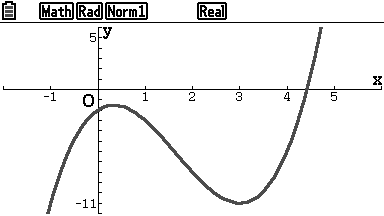
\includegraphics[scale=0.55]{assets/26-graph6.png}
          \end{vwcol}

          \begin{multicols}{2}
              \item $y = x^3 - 3x^2 + 4$
              \sol{}

              When $y = 0$,
              \begin{flalign*}
                  x^3 - 3x^2 + 4      & = 0               & \\
                  (x+1)(x^2 - 4x + 4) & = 0               & \\
                  (x+1)(x-2)^2        & = 0               & \\
                  x = -1              & \text{ or } x = 2
              \end{flalign*}
              $\therefore$ The $x$-intercepts are $(-1, 0)$ and $(2, 0)$.

              When $x = 0$, $y = 4$.

              $\therefore$ The $y$-intercept is $(0, 4)$.
              \begin{flalign*}
                  y'    & = 3x^2 - 6x       & \\
                  y''   & = 6x - 6          & \\
                  0     & = 3x^2 - 6x       & \\
                  0     & = x(x - 2)        & \\
                  x = 0 & \text{ or } x = 2
              \end{flalign*}
              When $x = 0$, $y'' = -6 < 0$.

              When $x = 2$, $y'' = 6 > 0$.

              $\therefore$ The function has a relative maximum point at $(0, 4)$ and a relative minimum point at $(2, 0)$.
              \begin{flalign*}
                  6x - 6 & = 0 & \\
                  x      & = 1
              \end{flalign*}
              When $x = 1$, $y = (1)^3 - 3(1)^2 + 4 = 2$.

              \noindent In the interval $(-\infty, 1)$, $y'' < 0$, hence the function is convex upward.

              \noindent In the interval $(1, \infty)$, $y'' > 0$, hence the function is convex downward.

              \noindent The point of inflection is $(1, 2)$.
              \vspace{2em}
              \begin{center}
                  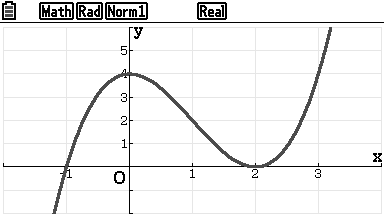
\includegraphics[scale=0.55]{assets/26-graph7.png}
              \end{center}
              \columnbreak

              \item In a container, the relationship between the volume of water $V$ (cm$^3$) and
              the depth of water $x$ (cm) is given by the equation $V = 4x^2 +
                  \dfrac{1}{6}x^3$. If the water is poured into the container at a rate of $6$
              cm$^3$ per second, find the rate of change of the depth of water when $x=2$ cm.
              \sol{}
              \begin{flalign*}
                  V              & = 4x^2 + \dfrac{1}{6}x^3                         & \\
                  \dfrac{dV}{dx} & = 8x + \dfrac{1}{2}x^2                           & \\
                  \dfrac{dV}{dt} & = 6                                              & \\
                  \dfrac{dx}{dt} & = \dfrac{dx}{dV} \cdot \dfrac{dV}{dt}            & \\
                                 & = \dfrac{1}{\dfrac{dV}{dx}} \cdot \dfrac{dV}{dt} & \\
                                 & = \dfrac{1}{8x + \dfrac{1}{2}x^2} \cdot 6        & \\
                                 & = \dfrac{6}{8x + \dfrac{1}{2}x^2}
              \end{flalign*}
              When $x = 2$,
              \begin{flalign*}
                  \dfrac{dx}{dt} & = \dfrac{6}{8(2) + \dfrac{1}{2}(2)^2} & \\
                                 & = \dfrac{6}{18}                       & \\
                                 & = \dfrac{1}{3} \text{ cm s}^{-1}
              \end{flalign*}
          \end{multicols}

          \newpage
    \item The water is poured into a conical pool with a height and a base radius of
          $20$m and $10$m respectively at a rate of $5$m$^3$/min. When the height of the
          water is $10$m, find
          \begin{enumerate}
              \item the rate of increasing of the height of the water. \sol{}

                    Let the height of the water be $h$cm and the radius of the water surface be
                    $r$cm.
                    \begin{flalign*}
                        \dfrac{h}{20}  & = \dfrac{r}{10}                                  & \\
                        r              & = \dfrac{h}{2}                                   & \\
                        V              & = \dfrac{1}{3}\pi r^2 h                          & \\
                                       & = \dfrac{1}{3}\pi \left(\dfrac{h}{2}\right)^2 h  & \\
                                       & = \dfrac{1}{12}\pi h^3                           & \\
                        \dfrac{dV}{dh} & = \dfrac{1}{4}\pi h^2                            & \\
                        \dfrac{dV}{dt} & = 5                                              & \\
                        \dfrac{dh}{dt} & = \dfrac{dh}{dV} \cdot \dfrac{dV}{dt}            & \\
                                       & = \dfrac{1}{\dfrac{dV}{dh}} \cdot \dfrac{dV}{dt} & \\
                                       & = \dfrac{1}{\dfrac{1}{4}\pi h^2} \cdot 5         & \\
                                       & = \dfrac{20}{\pi h^2} \text{ m min}^{-1}
                    \end{flalign*}
                    When $h = 10$,
                    \begin{flalign*}
                        \dfrac{dh}{dt} & = \dfrac{20}{\pi (10)^2}             & \\
                                       & = \dfrac{1}{5\pi} \text{ m min}^{-1}
                    \end{flalign*}

              \item the rate of change of the area of the water surface. \sol{}
                    \begin{flalign*}
                        A              & = \pi r^2                         & \\
                                       & = \pi \left(\dfrac{h}{2}\right)^2 & \\
                                       & = \dfrac{1}{4}\pi h^2             & \\
                        \dfrac{dA}{dh} & = \dfrac{1}{2}\pi h
                    \end{flalign*}
                    When $h = 10$,
                    \begin{flalign*}
                        \dfrac{dh}{dt} & = \dfrac{1}{5\pi}                            & \\
                        \dfrac{dA}{dt} & = \dfrac{dA}{dh} \cdot \dfrac{dh}{dt}        & \\
                                       & = \dfrac{1}{2}\pi (10) \cdot \dfrac{1}{5\pi} & \\
                                       & = 1 \text{ m}^2 \text{ min}^{-1}
                    \end{flalign*}
          \end{enumerate}

    \item The radius of a spherical container decreases from $4$cm to $3.95$cm. Find the
          approximate amount of decrease in the volume and the surface area of the
          container. \sol{}
          \begin{flalign*}
              V                          & = \dfrac{4}{3}\pi r^3     & \\
              A                          & = 4\pi r^2                & \\
              \dfrac{dV}{dr}             & = 4\pi r^2                & \\
              \dfrac{dA}{dr}             & = 8\pi r                  & \\
              \dfrac{\Delta V}{\Delta r} & = \dfrac{dV}{dr}          & \\
              \Delta V                   & = 4\pi r^2 \cdot \Delta r & \\
              \dfrac{\Delta A}{\Delta r} & = \dfrac{dA}{dr}          & \\
              \Delta A                   & = 8\pi r \cdot \Delta r
          \end{flalign*}
          When $r = 4$,$\Delta r = -0.05$,
          \begin{flalign*}
              \Delta V & = 4\pi (4)^2 (-0.05)   & \\
                       & = -3.2\pi \text{ cm}^3 & \\
              \Delta A & = 8\pi (4)(-0.05)      & \\
                       & = -1.6\pi \text{ cm}^2
          \end{flalign*}
          $\therefore$ The approximate amount of decrease in the volume and the surface area of the container is $-3.2\pi$cm$^3$ and $-1.6\pi$cm$^2$ respectively.
          \vfill\null

    \item The capacity of water of a spherical container is given by $V =
              \left[\dfrac{\pi h^2}{3}(15-h)\right]$cm$^3$, where $h$ is the depth of the
          water. Find the approximate amount of increase in the capacity of the container
          when the depth of the water increases from $4$cm to $4.01$cm. \sol{}
          \begin{flalign*}
              V                          & = 5\pi h^2 - \dfrac{1}{3}\pi h^3     & \\
              \dfrac{dV}{dh}             & = 10\pi h - \pi h^2                  & \\
              \dfrac{\Delta V}{\Delta h} & = \dfrac{dV}{dh}                     & \\
              \Delta V                   & = (10\pi h - \pi h^2) \cdot \Delta h &
          \end{flalign*}
          When $h = 4$,$\Delta h = 0.01$,
          \begin{flalign*}
              \Delta V & = (10\pi (4) - \pi (4)^2) \cdot 0.01 & \\
                       & = 0.24\pi \text{ cm}^3
          \end{flalign*}
          $\therefore$ The approximate amount of increase in the capacity of the container is $0.24\pi$cm$^3$.
          \vfill\null

          \newpage

    \item In a bowl, when the height of the water is $h$cm, the volume of the water is
          given by $V = \left(h^3 + 3h^2 + 11h\right)$cm$^3$. When the height of the
          water is $7cm$, pour an additional $\Delta V$cm$^3$ of water into the bowl.
          Find the approximate amount of increase in the height of the water. \sol{}
          \begin{flalign*}
              \dfrac{dV}{dh}             & = 3h^2 + 6h + 11                   & \\
              \dfrac{\Delta V}{\Delta h} & = \dfrac{dV}{dh}                   & \\
              \Delta V                   & = (3h^2 + 6h + 11) \cdot \Delta h  & \\
              \Delta h                   & = \dfrac{\Delta V}{3h^2 + 6h + 11}
          \end{flalign*}
          When $h = 7$,
          \begin{flalign*}
              \Delta h & = \dfrac{\Delta V}{3(7)^2 + 6(7) + 11} & \\
                       & = \dfrac{\Delta V}{200} \text{ cm}
          \end{flalign*}
          $\therefore$ The approximate amount of increase in the height of the water is $\dfrac{\Delta V}{200}$cm.

    \item If $y = \dfrac{1}{\sqrt[3]{x}}$, find $\dfrac{dy}{dx}$. Hence, find the
          approximate value of $\dfrac{1} {\sqrt[3]{130}}$. (Correct to 3 decimal places)
          \sol{}
          \begin{flalign*}
              y                          & = x^{-\frac{1}{3}}                             & \\
              \dfrac{dy}{dx}             & = -\dfrac{1}{3}x^{-\frac{4}{3}}                & \\
              \dfrac{\Delta y}{\Delta x} & = \dfrac{dy}{dx}                               & \\
              \Delta y                   & = -\dfrac{1}{3}x^{-\frac{4}{3}} \cdot \Delta x
          \end{flalign*}
          When $x = 125$, $\Delta x = 5$,
          \begin{flalign*}
              \Delta y & = -\dfrac{1}{3}(125)^{-\frac{4}{3}} \cdot 5 & \\
                       & = -0.003
          \end{flalign*}
          $\therefore$ The approximate value of $\dfrac{1} {\sqrt[3]{130}}$ is $\dfrac{1}{5} - 0.003 = 0.197$.
\end{enumerate}
